\subsection{Terzo test}

Sulla base dei risultati ottenuti nei test precedenti, si esegue un'ultima analisi per verificare
quanti campioni siano necessari per ridurre al minimo la discrepanza tra le reti generate e quella
di partenza, misurando anche il tempo necessario. Per fare ciò si utilizza lo script
\texttt{min\_diff.py} che genera insiemi di campioni di cardinalità $1000 \cdot 2^x$ con $1 \le x
    \le 8$ sui quali viene eseguito l'algoritmo di apprendimento tramite l'euristica logaritmica (dato
che quella fattoriale fallisce dopo 160 campioni).

\subsubsection{Risultati}

\begin{figure}[h]
    \centering
    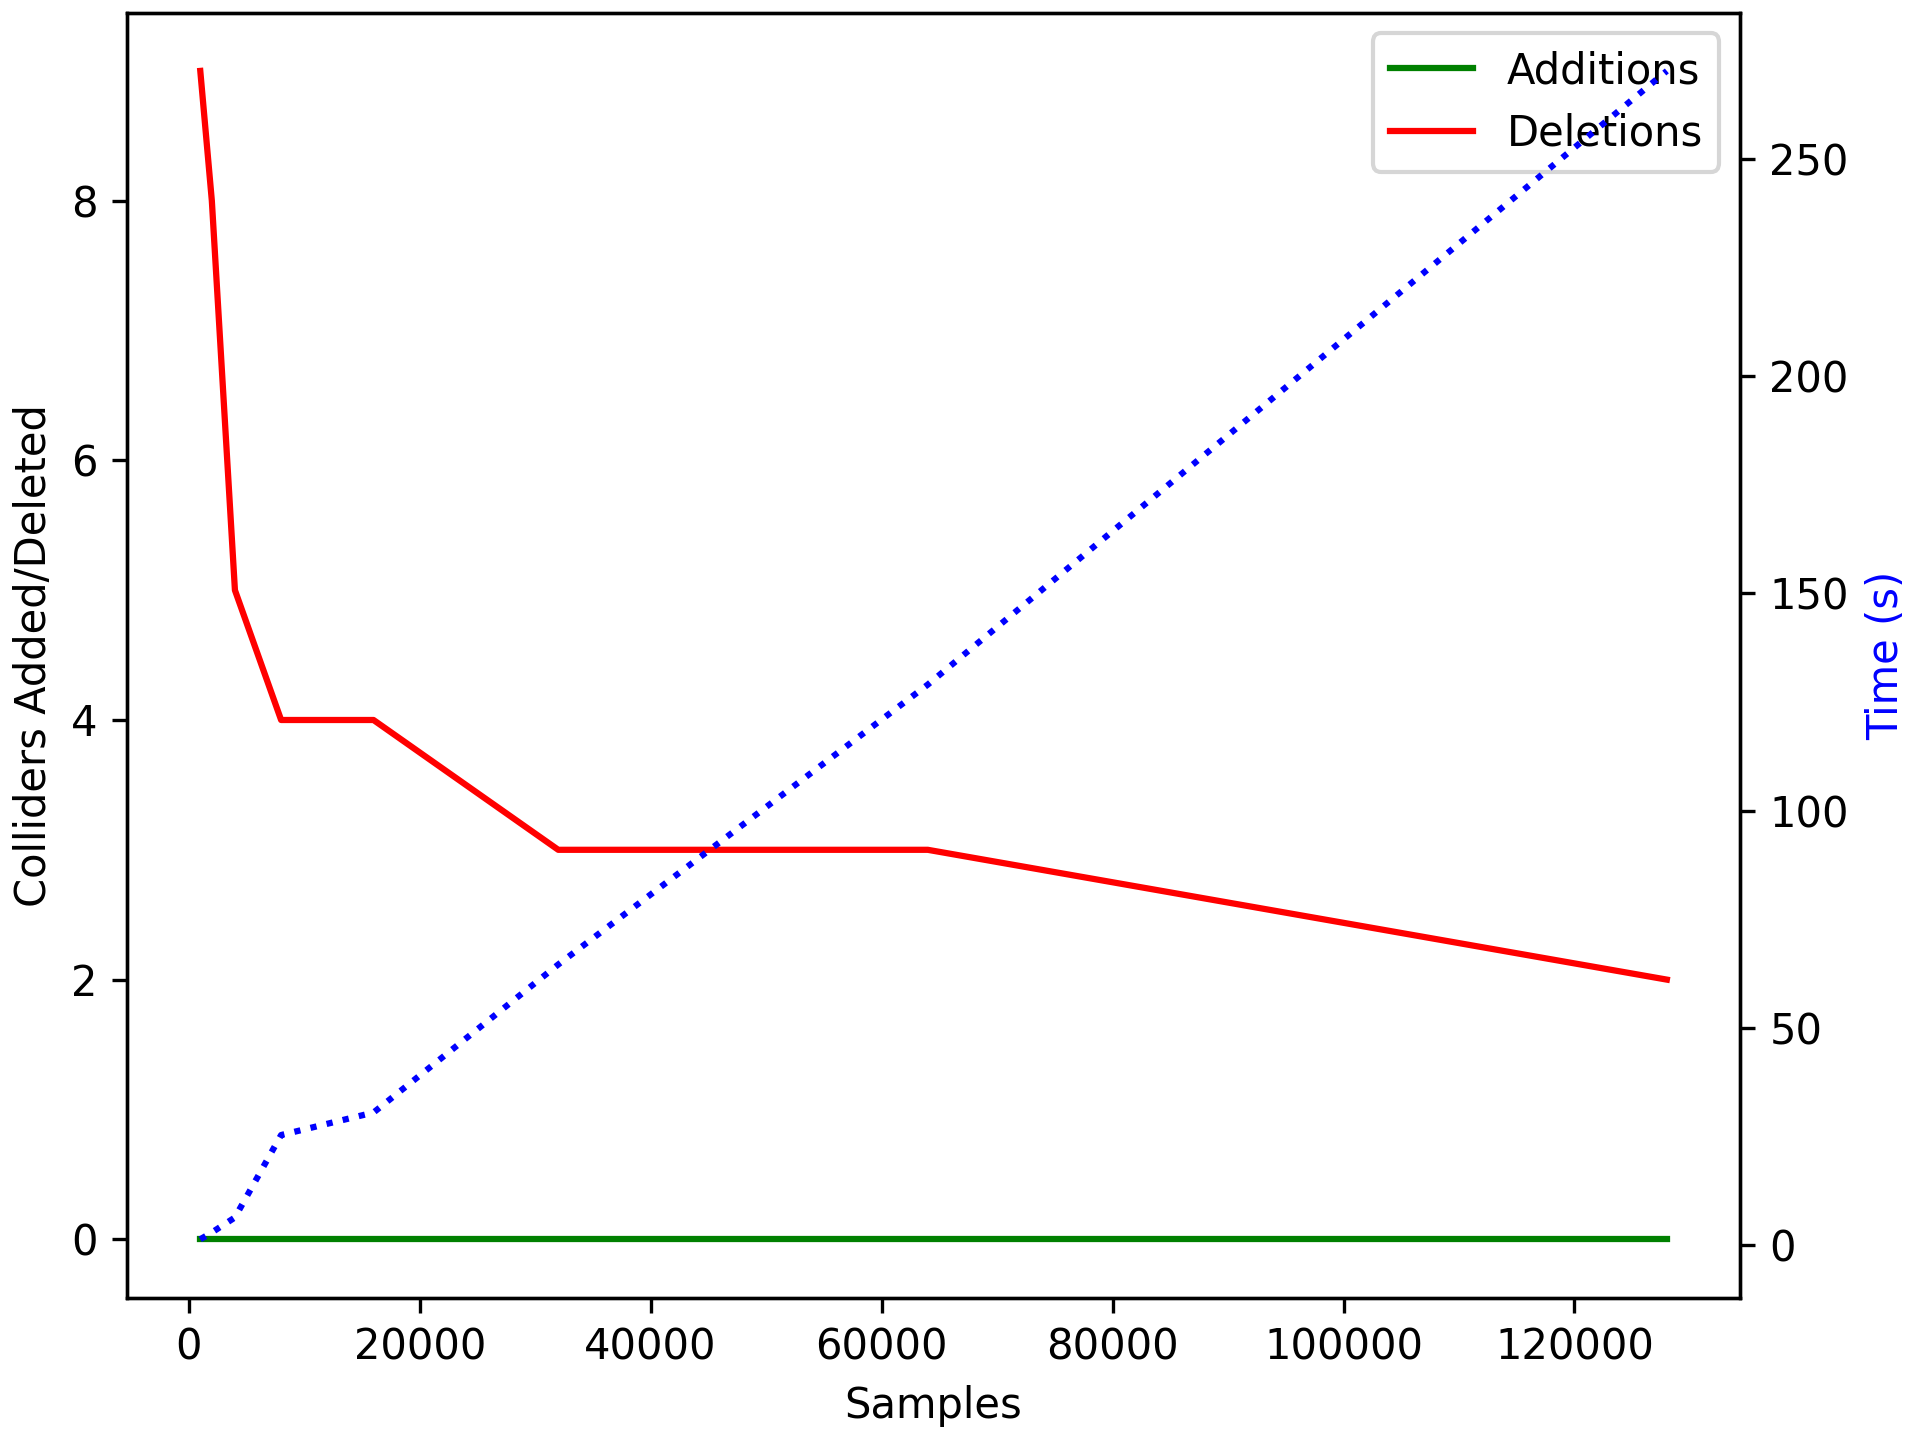
\includegraphics[width=0.6\textwidth]{min_diff.png}
    \caption{relazione tra il numero di collider errati e il numero di campioni; sull'ordinata destra è indicato il tempo di esecuzione}
    \label{fig:test3}
\end{figure}

Si può notare che nonostante un numero esponenziale di campioni, la rete generata non risulta
identica a quella di partenza da cui è stata generata la distribuzione, infatti il numero di
collider in eccesso raggiunge lo zero, ma il numero di collider in difetto diminuisce in maniera
molto lenta. Questo può indicare che l'algoritmo cerca di approssimare la rete ad una rete più
"\textit{libera}" che contiene meno dipendenze condizionali. Si è preferito fermarsi a 128000
campioni in quanto oltre tale soglia i tempi di esecuzione diventano superiori ai 5 minuti.
